\section{Results}

\subsection{Experimental setup}

\subsubsection{\emph{Datasets}}

\paragraph{MMLU-Pro}
In this study, we utilize the MMLU-Pro dataset~\cite{wang2025mmlu}, a more challenging and robust variant of the well-known Massive Multitask Language Understanding (MMLU) benchmark. The original MMLU dataset was introduced by Hendrycks et al.~\cite{hendrycks2020measuring} and has been widely used to evaluate language model performance across diverse domains. MMLU-Pro builds upon this benchmark by incorporating a filtered and refined subset of the original questions, also introducing newly generated question-answer pairs to enhance difficulty and robustness.

The dataset consists of approximately $12000$ multiple-choice questions, with $10$ answer choices per question in the majority of cases (approximately $ 10000$ instances), while the remaining $ 2000$ instances contain between $3$ to $9$ answer options. 
The dataset spans 14 distinct scientific categories, covering a broad range of disciplines with the number of topics by discipline provided in Table~\ref{tab:mmlu_pro_distr}.
Examples of questions from different categories are available in Appendix~\ref{sec:question_examples}.

\begin{figure}
    \footnotesize\setlength{\tabcolsep}{2.8pt}
    \begin{tabular}{|c|c|c|}
    \hline
        Category & Sample Count \\
        \hline
        Mathematics & 1351 \\
        Physics & 1299 \\
        Chemistry & 1132 \\
        Law & 1101 \\
        Engineering & 969 \\
        Economics & 844 \\
        Health & 818 \\
        Psychology & 798 \\
        Business & 789 \\
        Biology & 717 \\
        Philosophy & 499 \\
        Computer Science & 410 \\
        History & 381 \\
        Other & 924 \\
        \hline
    \end{tabular}
    \captionof{table}{MMLU-Pro Category Distribution}
    \label{tab:mmlu_pro_distr}
\end{figure}

The motivation for using MMLU-Pro for this problem is its increased difficulty and improved robustness compared to the original MMLU dataset. 
Official reports for Phi-4 and Mistral-Small-24B also used the extended dataset to mitigate data leakage.
Thus, MMLU-Pro is a reliable and appropriate benchmark for evaluating our models' generalization and reasoning capabilities.

\subsubsection{\emph{Models.}} For QA and evaluation of the entropy, we use decoder-only LLMs Mistral (\textit{Mistral-Small-24B-Base-2501})~\cite{jiang2023mistral}, Phi-4~\cite{abdin2024phi} and Qwen models~\cite{qwen2025qwen25technicalreport}. 

\subsection{Reasoning and knowledge-based complexity}

We hypothesize that different questions validate different abilities of a model. Some focus more on the requirement to know specific things, while others consider a model's ability to reason within a specific topic.  

To obtain these properties for specific questions, we obtained estimates via the model-as-judge.
Figures \ref{fig:reasoning_distribution} present the question type by the requirement to reason and the estimate for the required number of reasoning steps.

The distribution of questions over topics is diverse, with the reasoning requirement attaining the maximum share of about $0.9$ for engineering and only $0.5$ for philosophy. The number of required steps also varies: again, for engineering, the model estimates the number of questions with a high number of required steps, but for psychology and philosophy, this number is almost zero.

\begin{figure}[t!]
    \centering
    \begin{subfigure}[t]{0.5\textwidth}
        \centering
        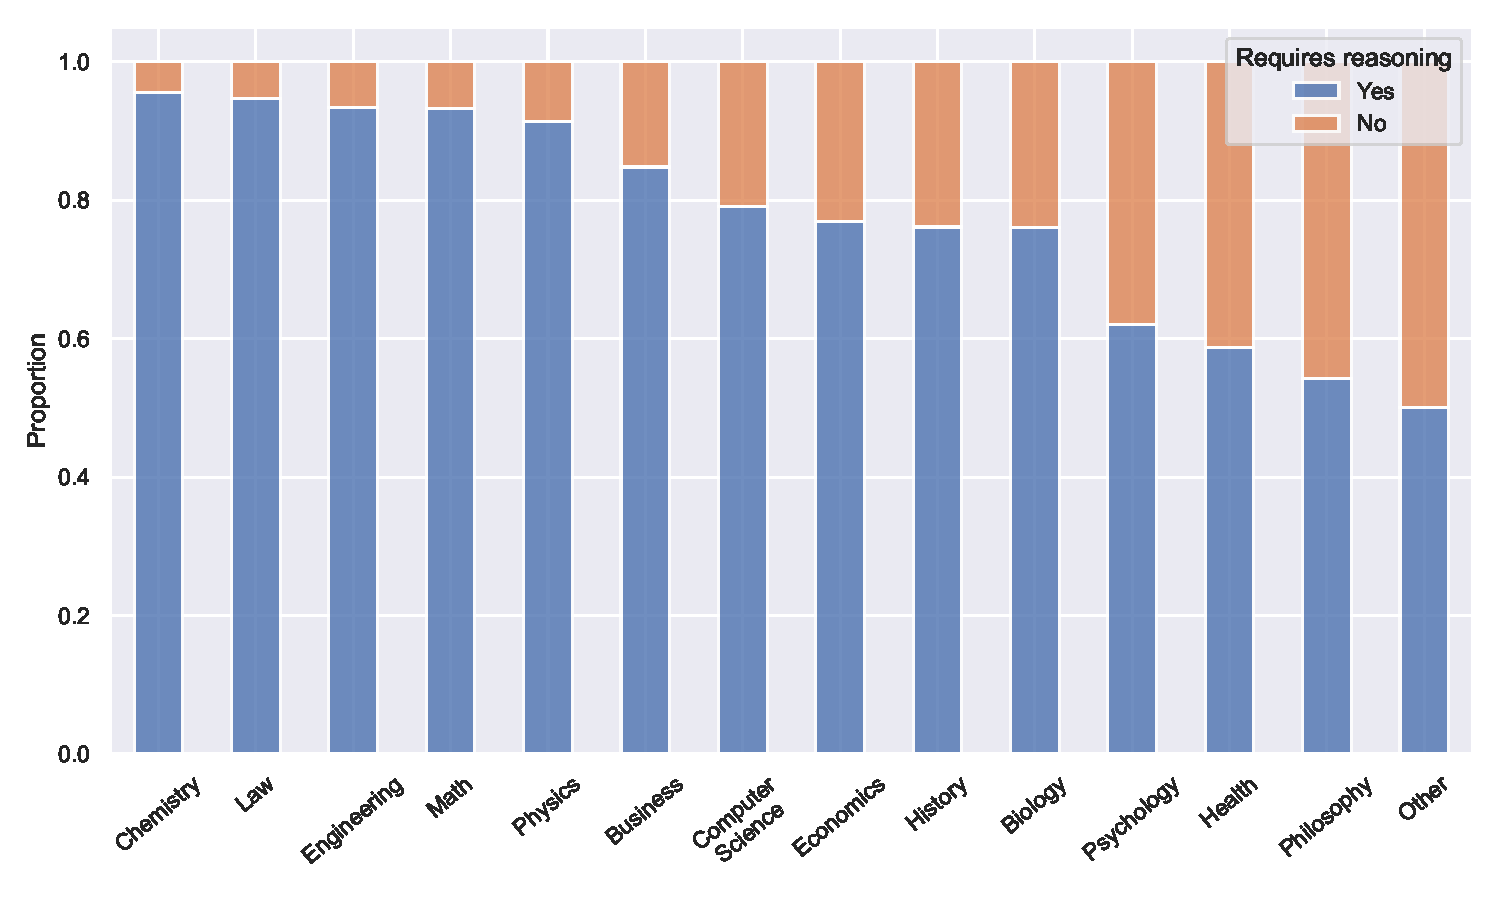
\includegraphics[width=\linewidth]{images/reasoning_binary.pdf}
        \caption{Distribution of questions that require complex reasoning}
    \end{subfigure}%
    ~ 
    \begin{subfigure}[t]{0.5\textwidth}
        \centering
        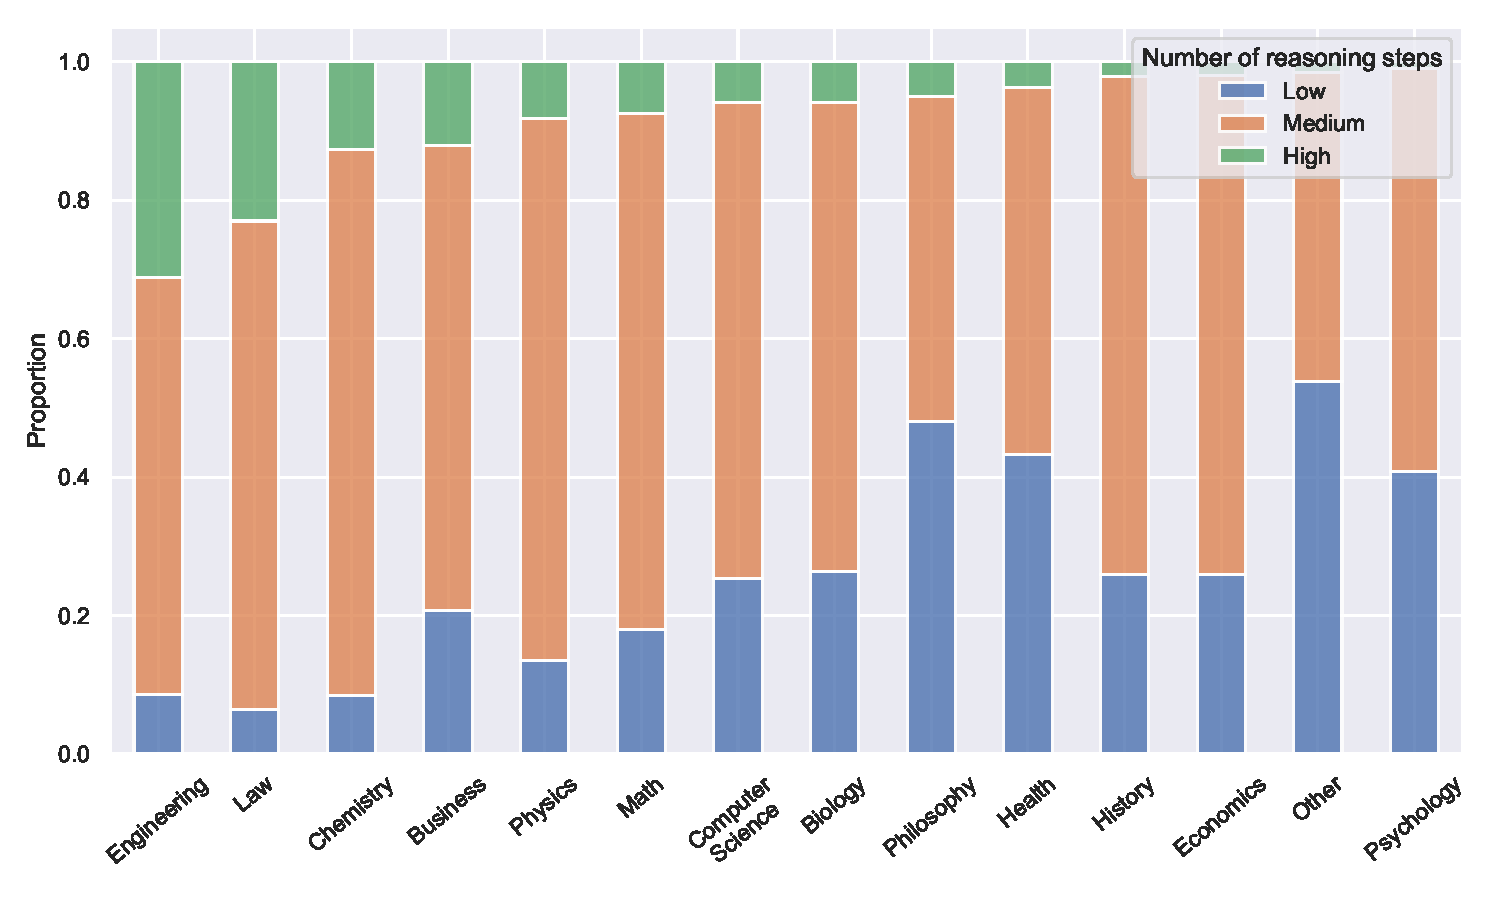
\includegraphics[width=\linewidth]{images/reasoning_levels.pdf}
        \caption{Distribution of the required number of reasoning steps}
    \end{subfigure}
    \caption{Estimation by MASJ of the required reasoning amount. Better to view in zoom}
    \label{fig:reasoning_distribution}
\end{figure}


\subsection{Distribution of uncertainty measures}

For Phi-4 and Qwen we present the distribution of entropy values in Figures~\ref{fig:entropy_distribution}.
The distribution of entropy is presented for correct and incorrect answers by a model. 
We can see near-zero entropy values are much more often observed for correct answers for Phi-4 and Qwen. 
Thus, entropy only partially explains why the answers from a model are wrong, and the quality of this score depends on the model used.

Both numerical and nominal Model-as-judge scores also relate little to the complexity, as the corresponding measured ROC AUC values are $0.49$ for both models, indicating nearly random predictions.
Thus, MASJ uncertainty estimates focus on different aspects of an LLM's confidence, which is irrelevant to question complexity.

\begin{figure}[t!]
    \centering
    \begin{subfigure}[t]{0.5\textwidth}
        \centering
        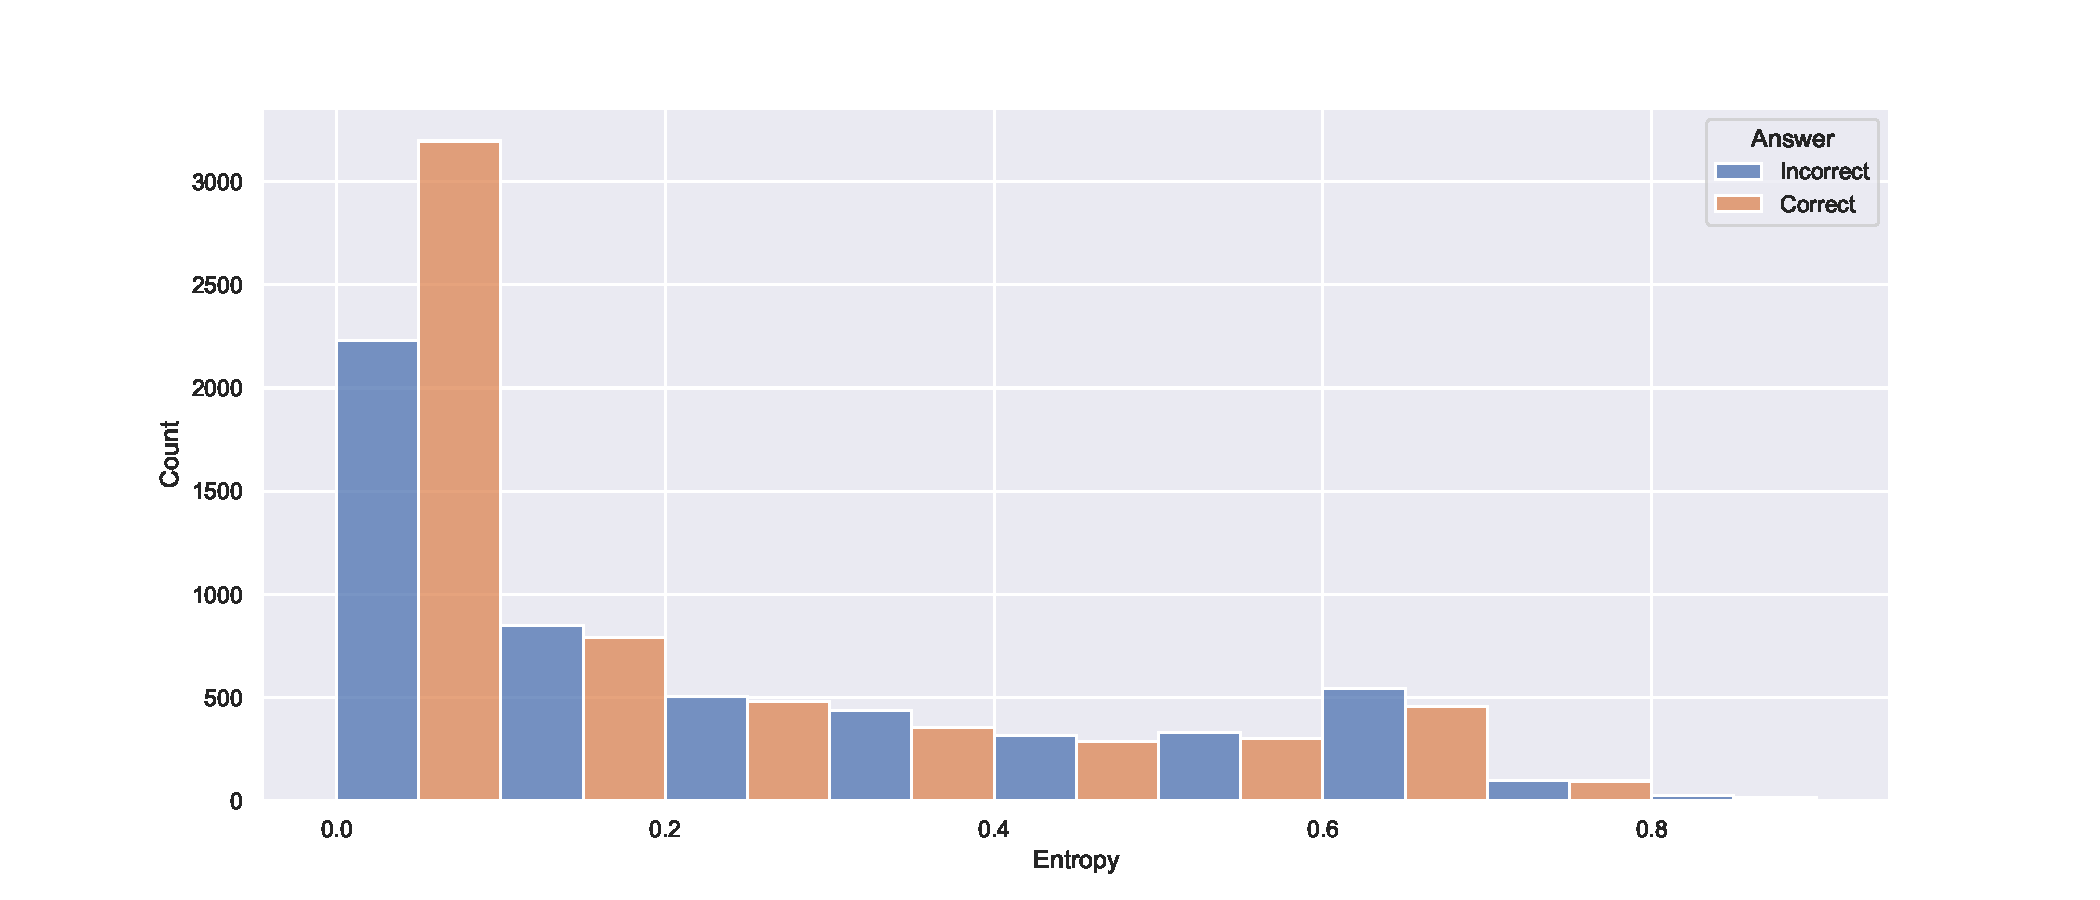
\includegraphics[width=\linewidth]{images/entropy_phi4.pdf}
        \caption{Phi-4 model} % A
    \end{subfigure}%
    ~ 
    \begin{subfigure}[t]{0.5\textwidth}
        \centering
        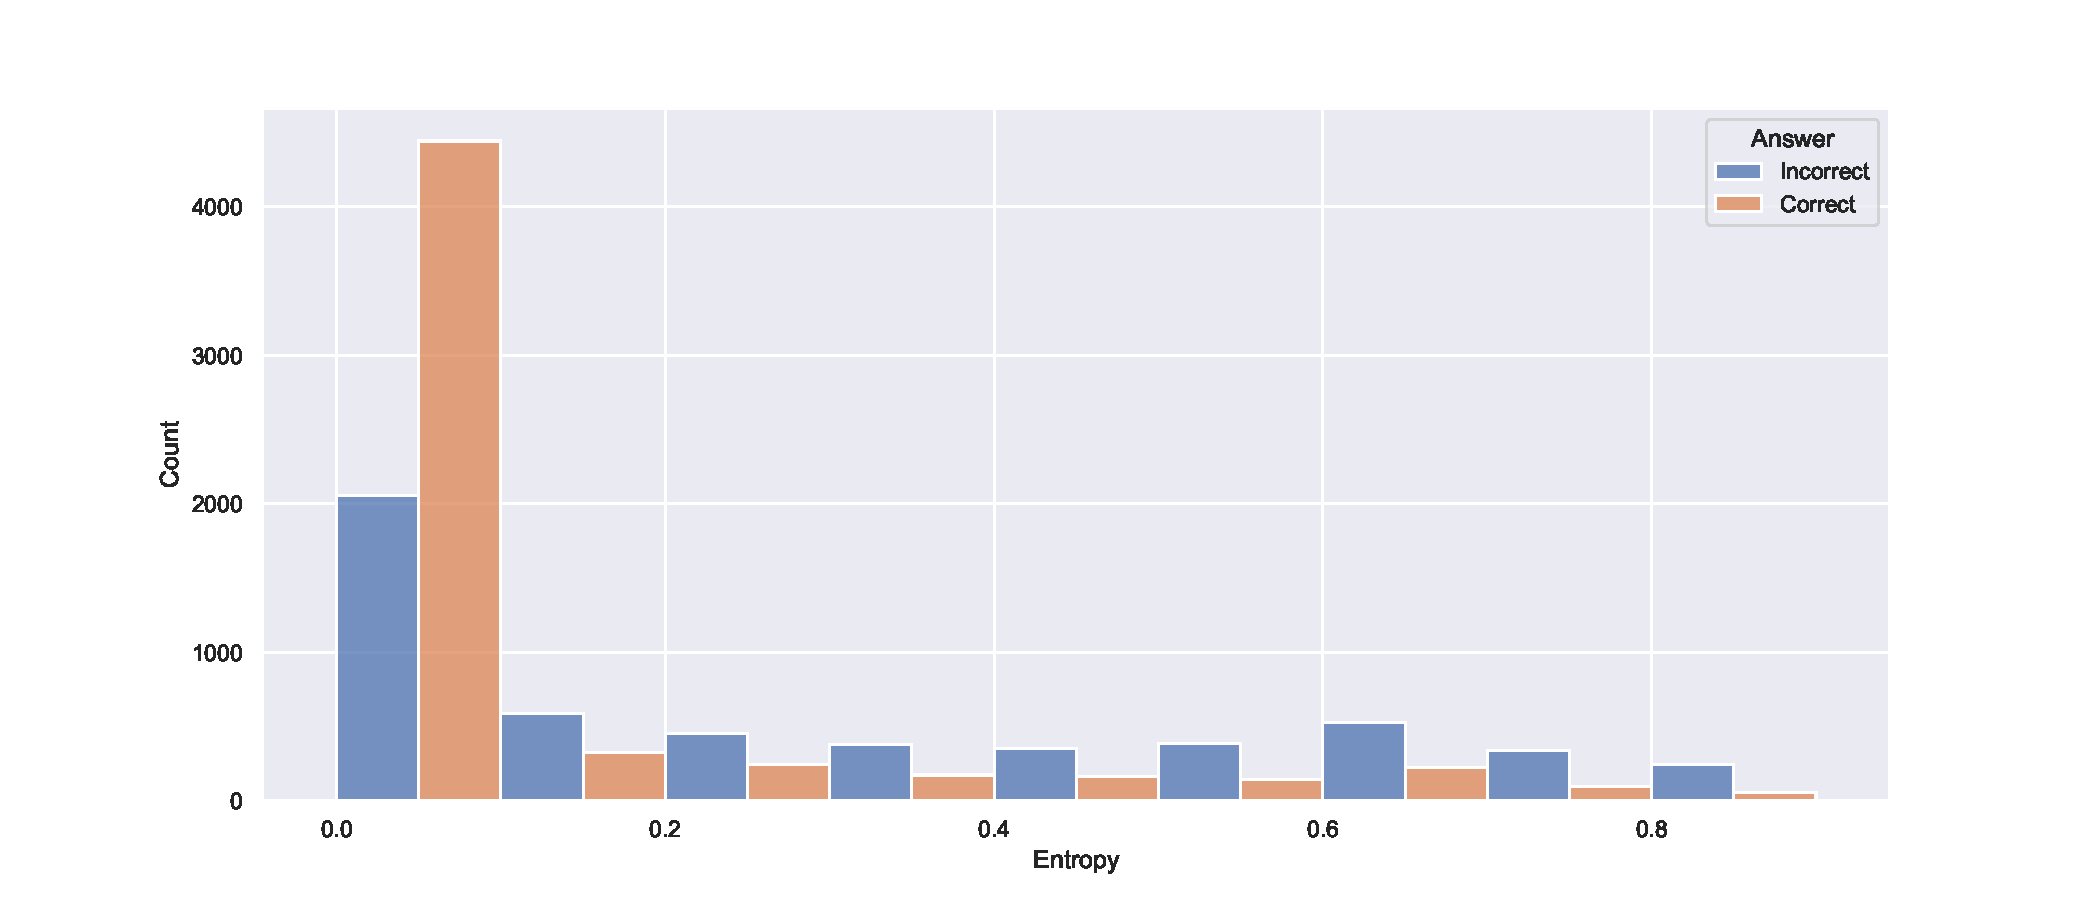
\includegraphics[width=\linewidth]{images/entropy_qwen72.pdf}
        \caption{Qwen-72B model} % B
    \end{subfigure}
    
    \vspace{1em}
    
    \centering
    \begin{subfigure}[t]{0.5\textwidth}
        \centering
        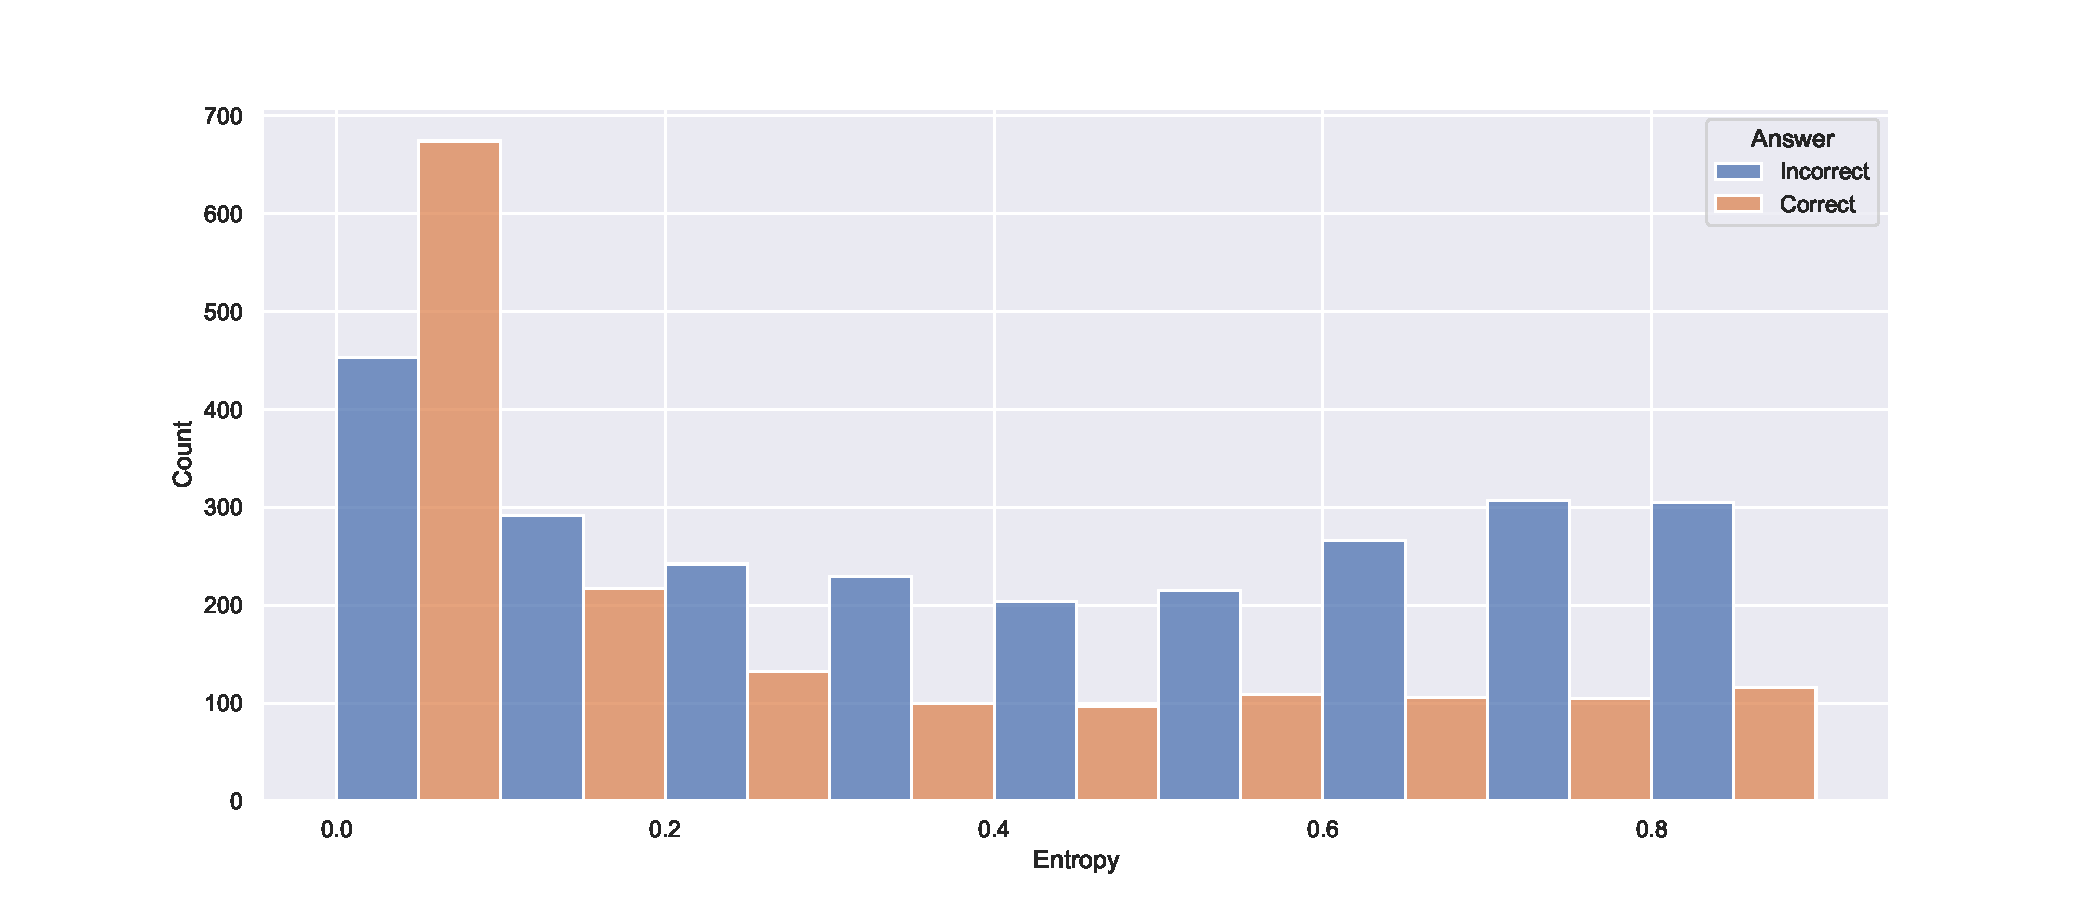
\includegraphics[width=\linewidth]{images/entropy_qwen1.5.pdf}
        \caption{Qwen-1.5B model} % C
    \end{subfigure}
    
    \caption{Entropy distribution of answers. Best viewed when zoomed in}
    \label{fig:entropy_distribution}
\end{figure}


\begin{figure}
    \centering
    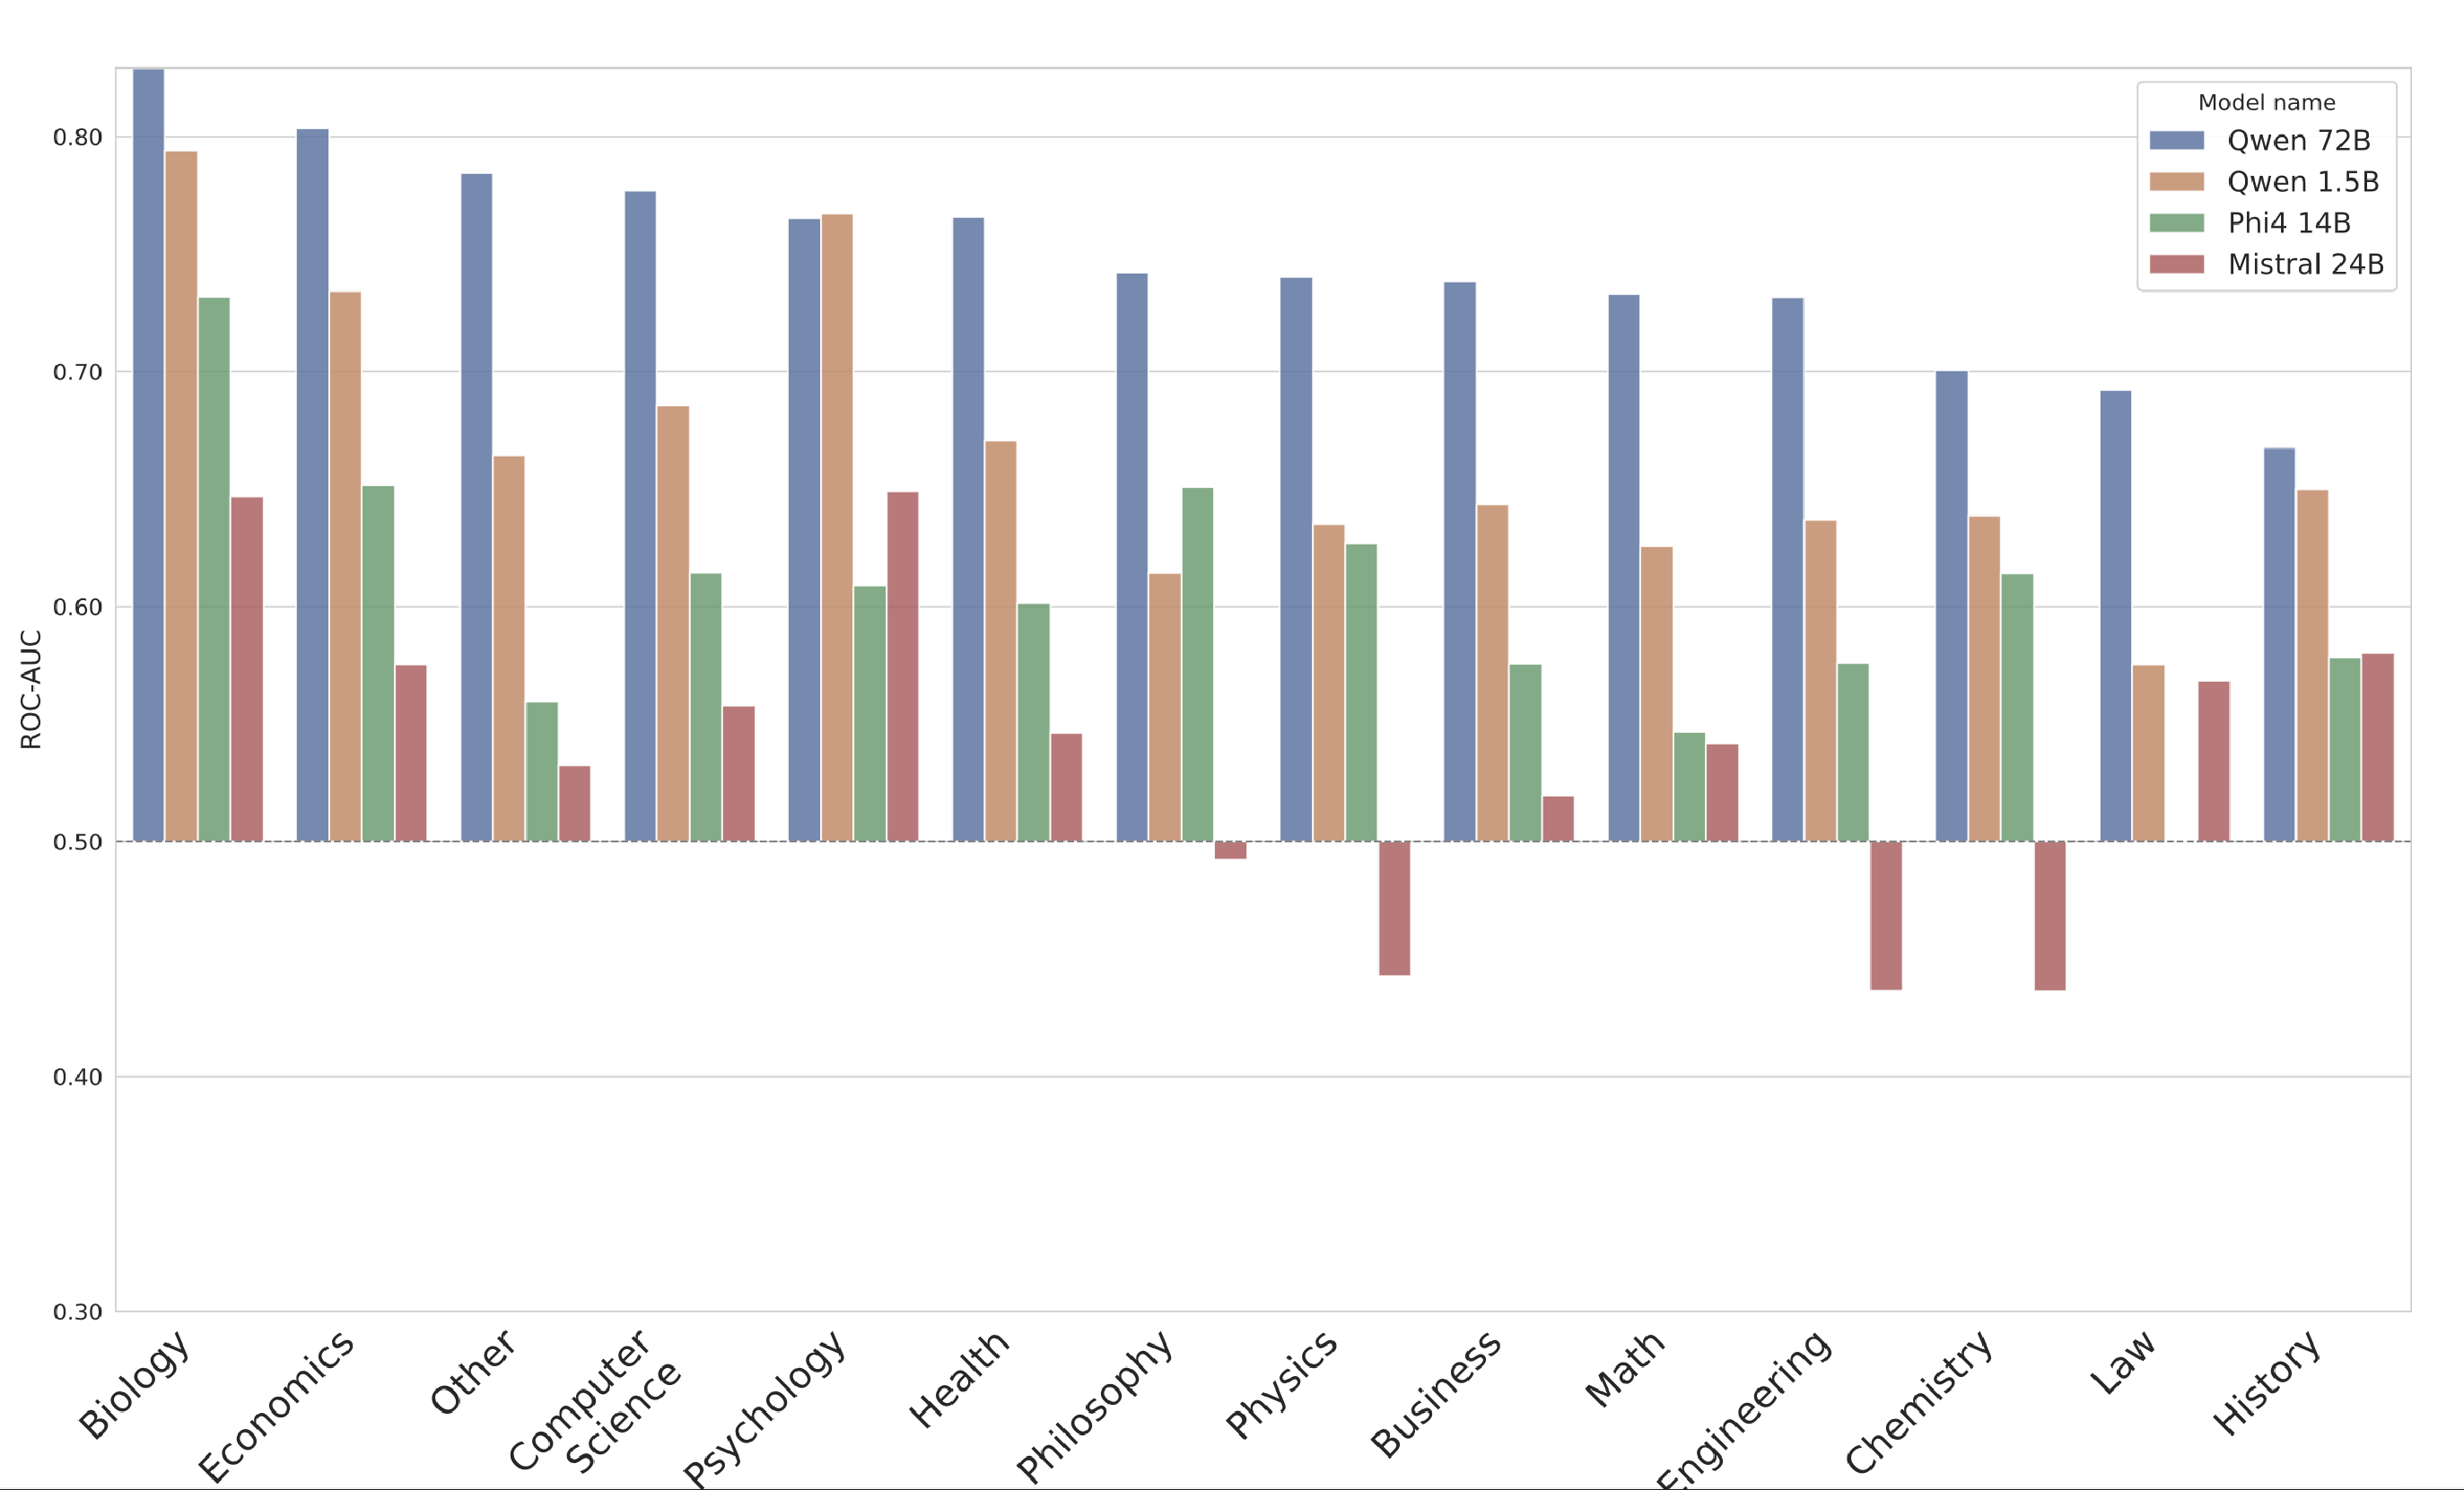
\includegraphics[width=1\linewidth]{images/models_compare_roc_auc.pdf}
    \caption{ROC-AUC for error prediction by subject for four different LLMs}
    % Qwen-72B, Qwen-1.5B, Phi4-14B, Mistral-24B}
    \label{fig:models_compare_roc_auc}
\end{figure}

\begin{table}[htbp]
\centering
\renewcommand{\arraystretch}{1.2}
\begin{tabular}{lcccc}
\hline
Category & Phi-4 & Mistral & Qwen 1.5B & Qwen 72B \\
\hline
Biology & \textbf{0.73} & \textbf{0.65} & \textbf{0.79} & \textbf{0.83} \\
Economics & 0.65 & 0.58 & 0.73 & 0.80 \\
Philosophy & 0.65 & \textit{0.49} & 0.61 & 0.74 \\
Physics & 0.63 & \textbf{0.44} & 0.64 & 0.74 \\
Computer Science & 0.61 & 0.56 & 0.69 & {0.78} \\
Psychology & 0.61 &\textbf{0.65} & 0.77 & 0.77 \\
Chemistry & 0.61 & 0.44 & 0.64 & 0.70 \\
Health & 0.60 & 0.55 & 0.67 & 0.77 \\
Business & 0.58 & 0.52 & 0.64 & 0.74 \\
History & 0.58 & 0.58 & 0.65 & \textit{0.67} \\
Engineering & 0.58 & 0.44 & 0.64 & 0.73 \\
Other & 0.56 & 0.53 & 0.66 & {0.78} \\
Math & 0.55 & 0.54 & 0.63 & 0.73 \\
Law & \textit{0.50} & 0.57 & \textit{0.58} & 0.69 \\
\hline
No Reasoning & \textbf{0.59} & \textbf{0.59} & \textbf{0.72} & \textbf{0.79} \\
Yes Reasoning & 0.56 & \textit{0.52} & 0.68 & 0.76 \\
Reasoning (Low) & \textbf{0.59} & 0.58 & 0.71 & \textbf{0.79} \\
Reasoning (Med) & 0.57 & \textit{0.52} & 0.69 & 0.76 \\
Reasoning (High) & \textit{0.53} & 0.53 & \textit{0.61} & \textit{0.73} \\
\hline
Overall & 0.58 & 0.52 & 0.70 & 0.77 \\
\hline
\end{tabular}
\caption{ROC AUC performance comparison across categories and models}
\label{tab:rocauc}
\end{table}

\subsection{Complexity prediction via uncertainty estimate by category and question type}

\paragraph{Complexity prediction by category.} Figure \ref{fig:models_compare_roc_auc} show the ROC-AUC values for entropy for all four models. Values above or below $0.5$ indicate that the prediction is better than random. For most topics, the values are well above this threshold. In psychology and biology, we observe ROC-AUC values of $0.77/0.83$ (Qwen 72B) compared to $0.61/0.73$ (Phi-4) and $0.65/0.65$ (Mistral), with these improvements correlating across models.

\paragraph{Complexity prediction by reasoning requirement.} 
Figure \ref{fig:models_compare_reasoning} present similar results, but for the split of the questions by reasoning complexity. Table \ref{tab:rocauc} shows aggregated ROC AUC scores across categories and reasoning levels. 

We see meaningful results of using the reasoning estimates for all questions without categorization by subject. Low entropy is a marginally better predictor of the truthfulness of the answers to questions that did not require complex reasoning and vice versa for models. We also observe the estimate of the number of reasoning steps as a less reliable metric, with Mistral favoring a higher number of reasoning steps. 
However, we can attribute it to the lower precision of such estimation provided by the MASJ approach. 

\begin{figure}
    \centering
    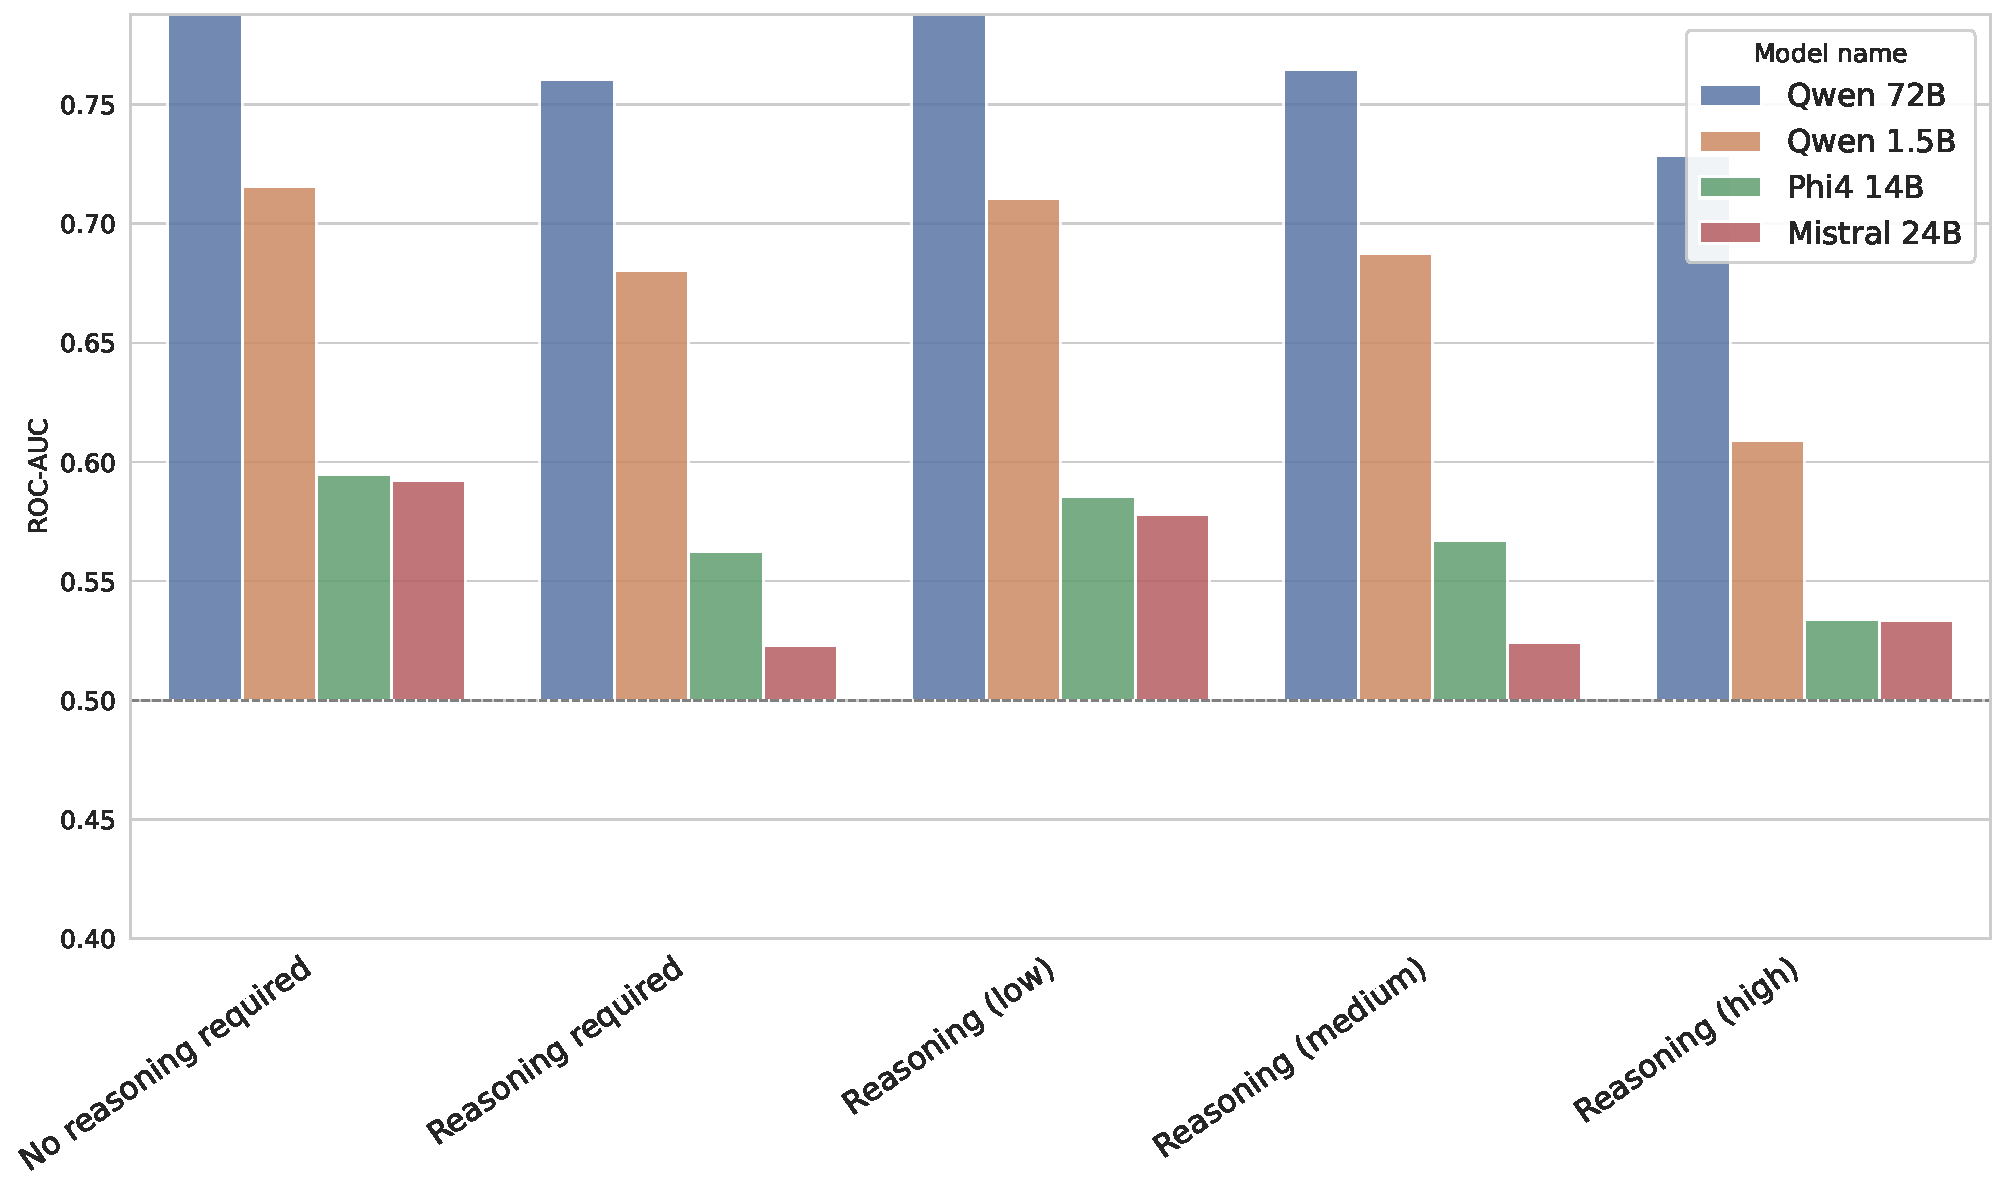
\includegraphics[width=1\linewidth]{images/models_compare_reasoning.pdf}
    \caption{ROC-AUC by reasoning for four different LLMs}
    \label{fig:models_compare_reasoning}
\end{figure}

\paragraph{Calibration assessment via entropy.}
Figure \ref{fig:models_compare_calibration} illustrates calibration curves for four language models, computed using inverted normalized entropy. The analysis reveals systematic deviations between self-reported certainty and empirical accuracy, with distinct patterns across architectures:

Mistral exhibits unstable calibration dynamics, characterized by erratic accuracy in low-confidence regions. Despite moderate confidence estimates, its accuracy fluctuates unpredictably, even peaking anomalously in the lowest entropy bin. This contrasts with its pronounced underperformance in high-confidence regimes, where empirical accuracy consistently trails reported certainty—a limitation indicative of architectural weaknesses in uncertainty quantification.

Qwen 72B, despite its large scale, demonstrates inconsistent calibration. High-confidence predictions show weak alignment with accuracy, while mid-range entropy bins display substantial confidence-accuracy gaps.

Qwen 1.5B emerges as an outlier, surpassing larger counterparts in calibration quality. Its confidence-accuracy relationship progresses monotonically across entropy bins, with minimal extreme deviations.

These results underscore systematic overconfidence as a pervasive issue, especially in high-certainty regimes where all models significantly overestimate their reliability.


\begin{figure}
    \centering
    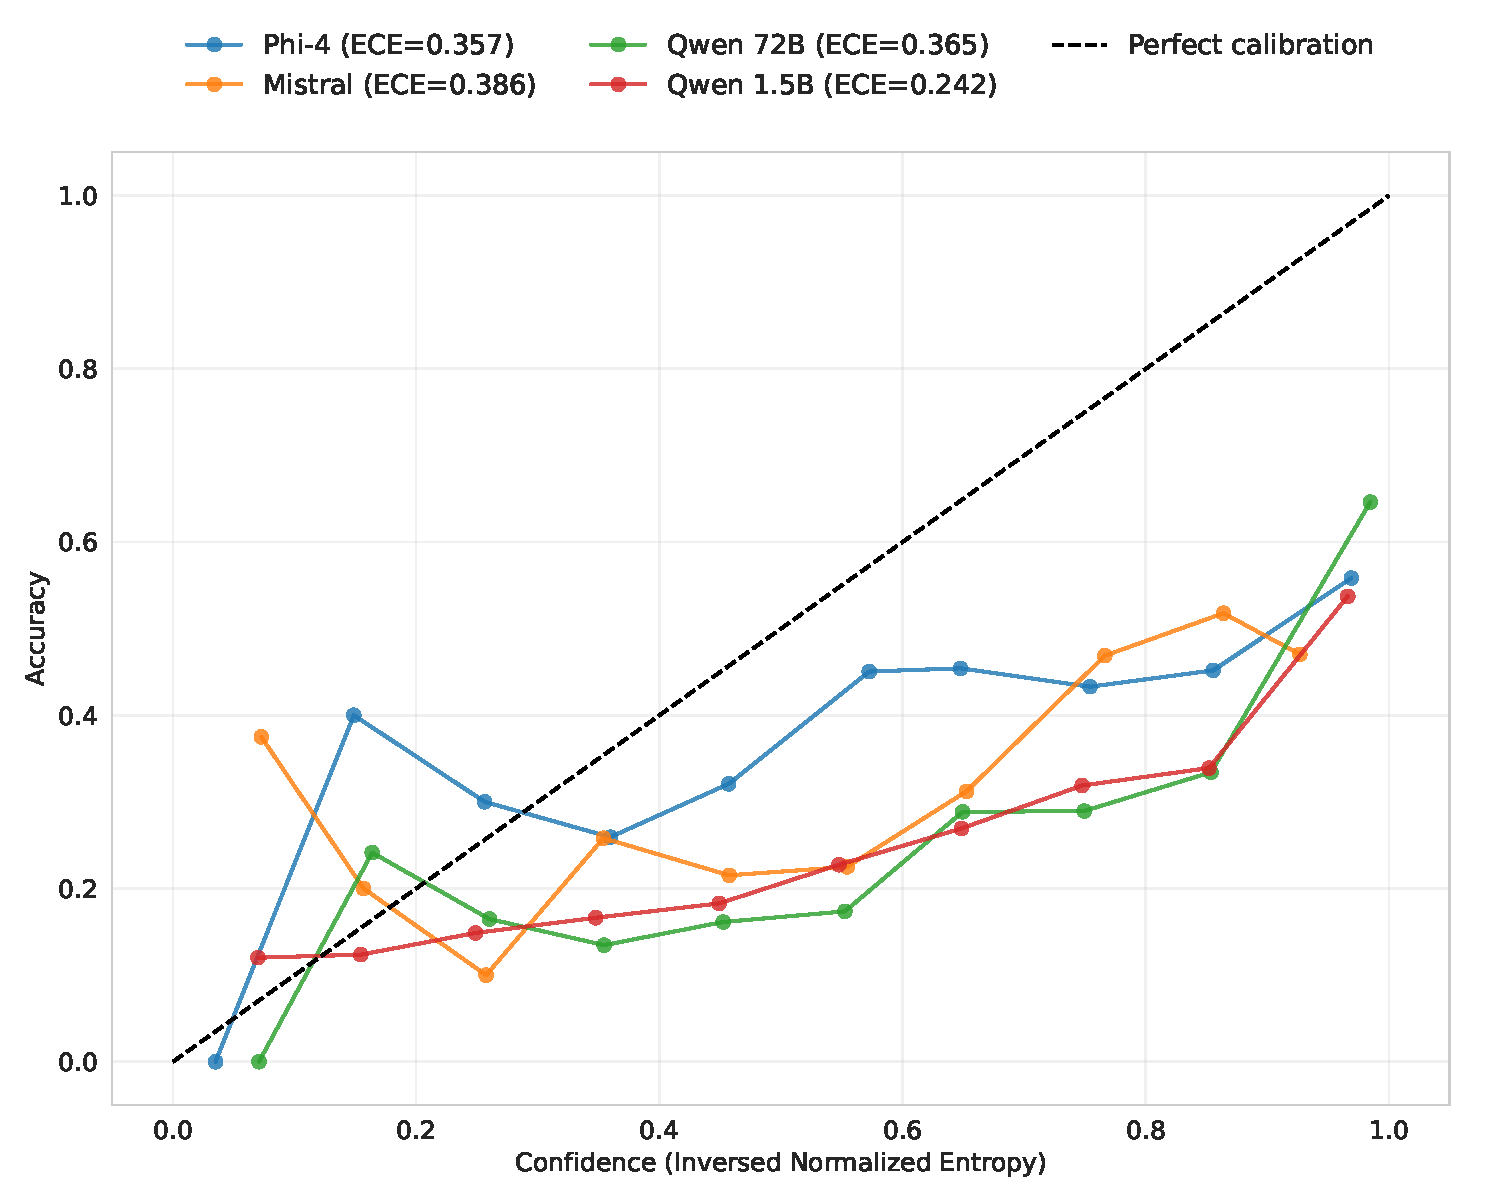
\includegraphics[width=1\linewidth]{images/models_compare_calibration.pdf}
    \caption{Calibration of LLMs based on their entropy}
    \label{fig:models_compare_calibration}
\end{figure}
